\problem{Image Restoration}
(a) The spectrum of the origin image is generated through FFT.\\
To shift the zero frequency to the center of the spectrum, we times $(-1)^{u+v}$ for each pixel $(u,v)$ on the origin image before applying FFT.

To have a better effect of visualization on the frequency domain, the image is shown by applying the log transformation on the magnitude of the Fourier transform of the image.\\
i.e. $I_{\text{log}}=20\log(1+|I|)$, where $I$ is the spectrum generated by Fourier transform of the image.

\begin{figure}[htbp]
    \centering
	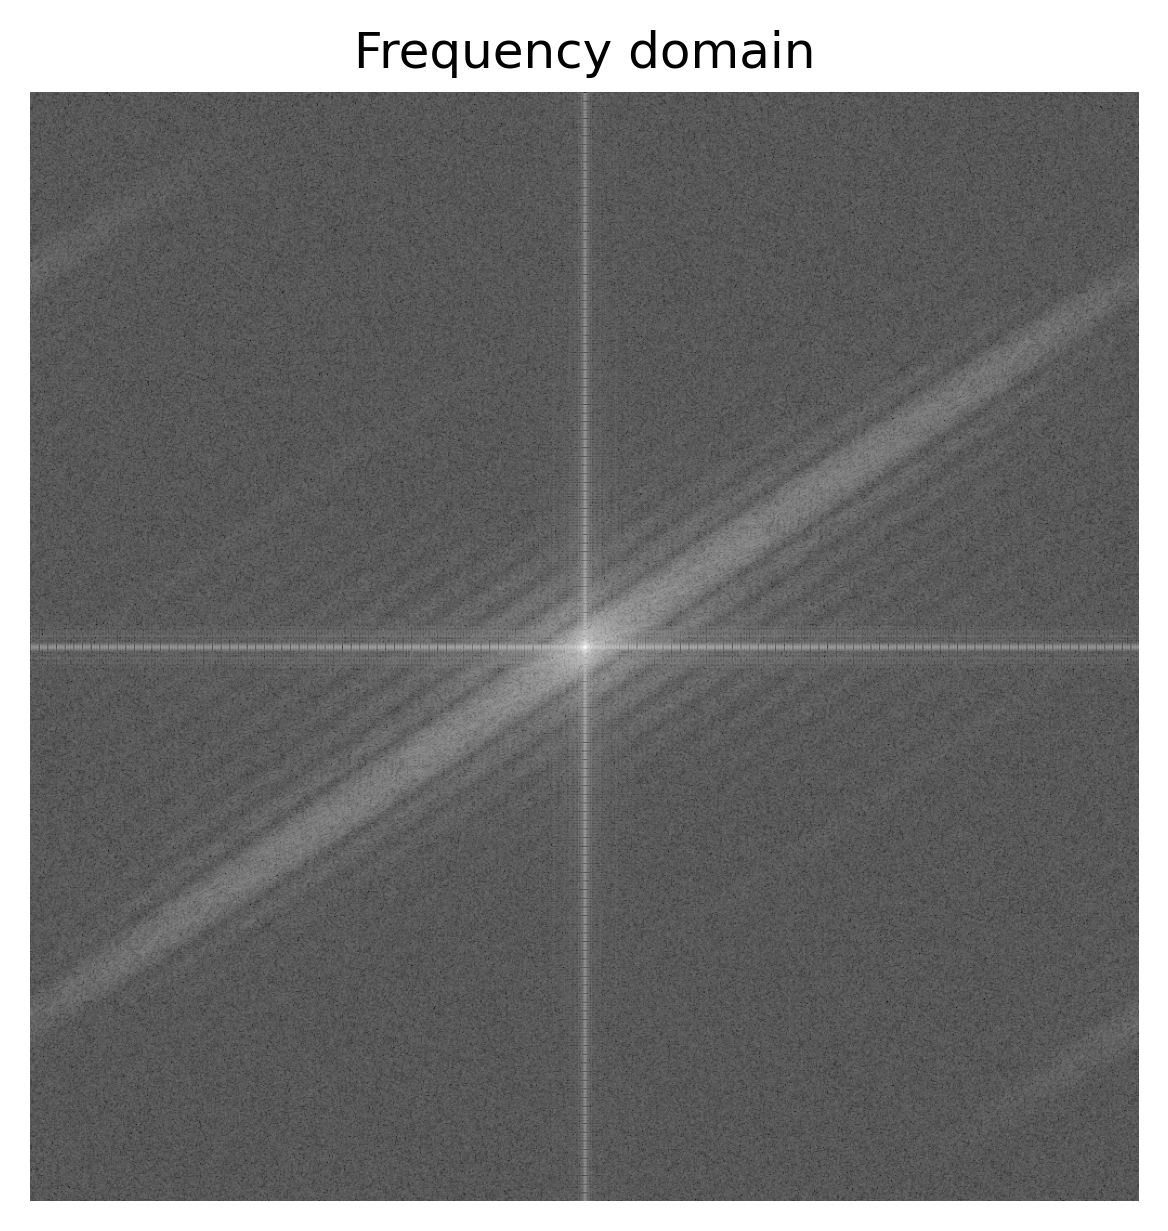
\includegraphics[width=0.5\textwidth]{../images/p4/p4a.png}
    \caption{FFT shifted spectrum}
    \label{fig:p4a}
\end{figure}

(b) The image by applying Radon transform on the origin image is shown in Figure \ref{fig:p4b}.\\
The Radon transform:
$$g(\rho, \theta)=\sum_{x=0}^{M-1}\sum_{y=0}^{N-1}f(x,y)\delta(x\cos\theta+y\sin\theta-\rho)$$
where $\delta$ is the Dirac delta function.\\

We can get the coordinates with the highest intensity in the Radon transformed image, which is $(\theta,d)=(,)$.\\

So above all, the angle between the strip and the vertical direction is $\theta=$
and the distance between two similar dark strips is $d=$

$N=640,L=\dfrac{N}{d}=$

\begin{figure}[htbp]
    \centering
	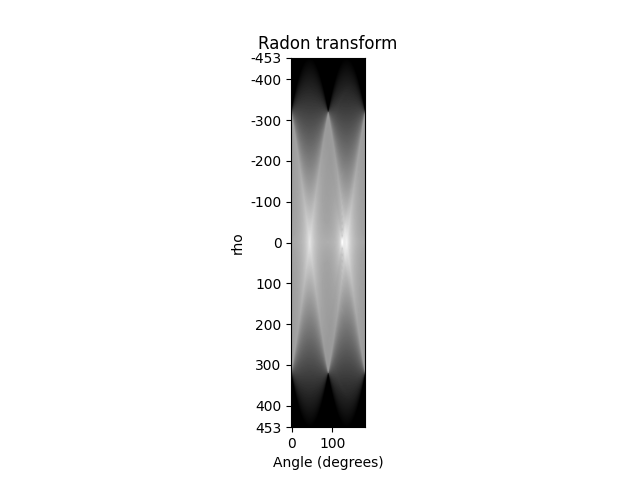
\includegraphics[width=\textwidth]{../images/p4/p4b_radon.png}
    \caption{Radon Transformed image}
    \label{fig:p4b}
\end{figure}

\begin{figure}[htbp]
    \centering
	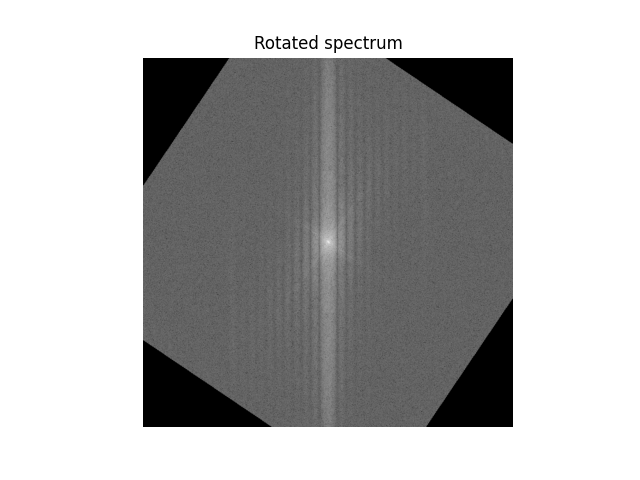
\includegraphics[width=\textwidth]{../images/p4/p4b_rotated_image.png}
	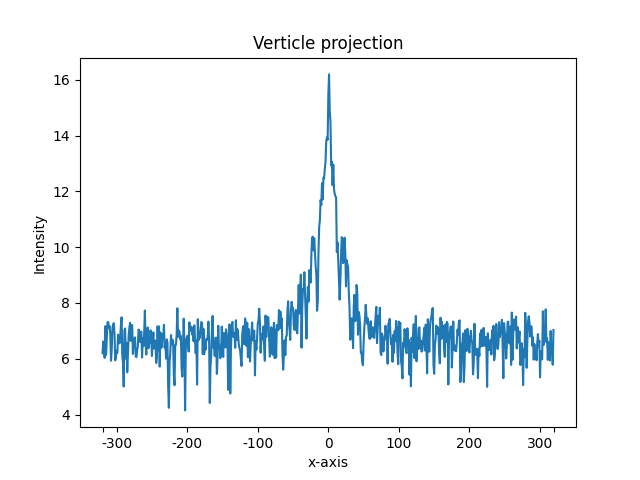
\includegraphics[width=\textwidth]{../images/p4/p4b_intensity.png}
    \caption{Radon Transformed image}
    \label{fig:p4b}
\end{figure}



(c)
We construct the frequency domain Wiener filter using the formula:
$$W = \dfrac{H^*}{|H|^2+\dfrac{S_n}{S_f}}$$
where $H$ is the Fourier transform of the point spread function, $S_n$ is the noise power spectrum, and $S_f$ is the signal power spectrum.\\
We here take $K=0.004$, and we do not apply `fftshift' during the filtering.

\begin{figure}[htbp]
    \centering
	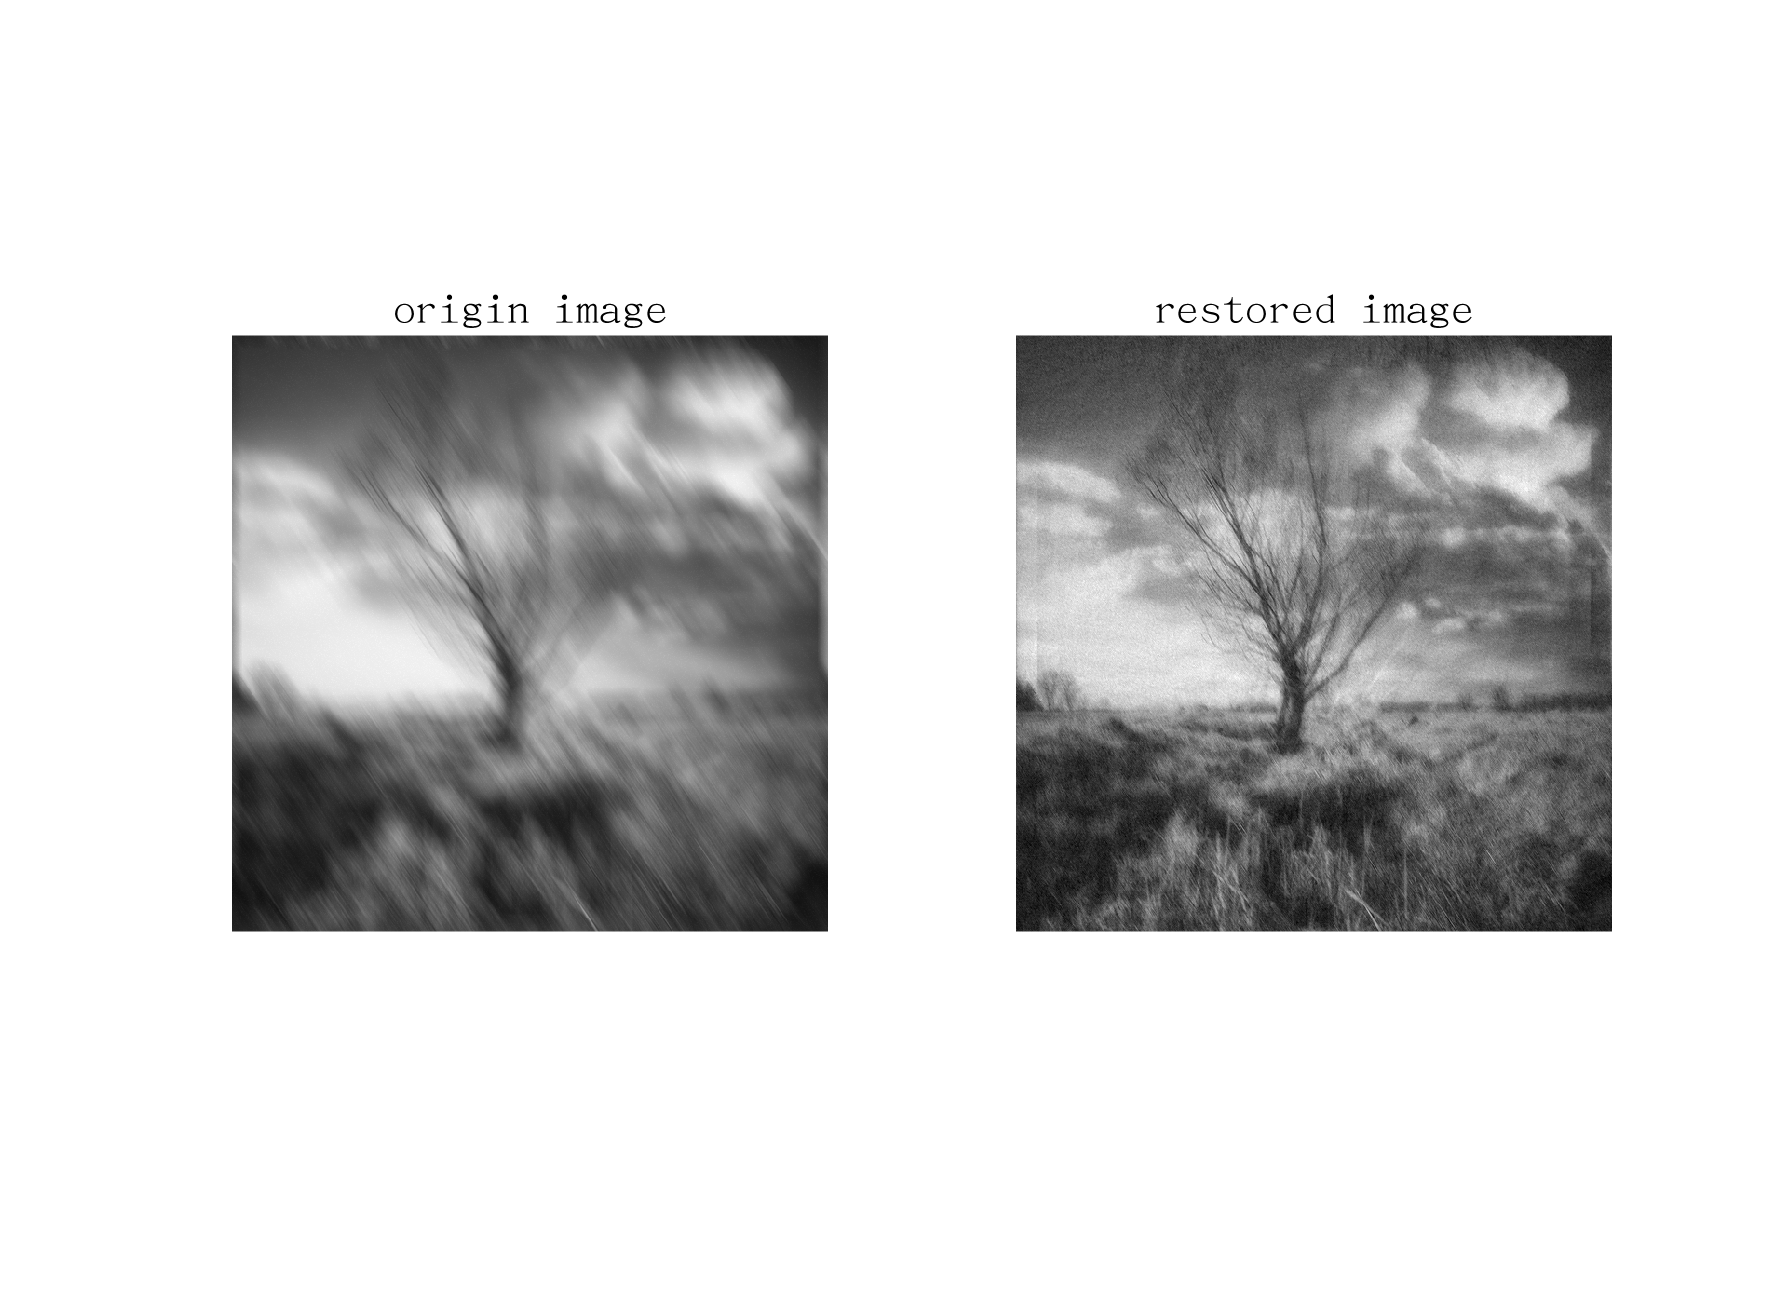
\includegraphics[width=\textwidth]{../images/p4/p4c.png}
    \caption{p4c}
    \label{fig:p4c}
\end{figure}




